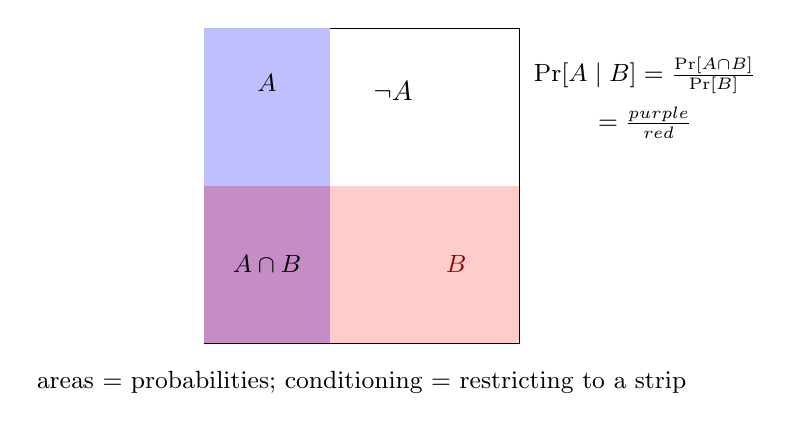
\begin{tikzpicture}[scale=1.0]
% unit square: x-axis A, y-axis B; A strip .4 wide, B band .5 tall, overlap = joint
\draw (0,0) rectangle (4,4);
\fill[blue!25] (0,0) rectangle (1.6,4);
\fill[red!20] (0,0) rectangle (4,2);
\fill[violet!45] (0,0) rectangle (1.6,2);
\node at (2.4,3.2) {$\neg A$};
\node at (0.8,3.3) {\small $A$};
\node[red!60!black] at (3.2,1.0) {\small $B$};
\node at (0.8,1.0) {\small $A\cap B$};
\node at (2,-0.5) {\small areas $=$ probabilities; conditioning $=$ restricting to a strip};
\node at (5.6,3.4) {\small $\Pr[A\mid B]=\frac{\Pr[A\cap B]}{\Pr[B]}$};
\node at (5.6,2.8) {\small $=\frac{\text{purple}}{\text{red}}$};
\end{tikzpicture}
